The purpose of this project is to analyse the electromagnetic signature of an object when its form changes during time. The electromagnetic signature analysis is a common subject for people who work in the field of radar detection. However, the study of object signature which form changes through time is still full of many questions remain in. The study of these objects imply a very strict analyse of the electronic signature thanks to the time frequency analysis tools.

\bigskip

During this project, we have to look at the different tools which can help us to analyse the electronic signature of an object and to help us to understand the effects of change of form of an object. The final deliverable expected is a set of programs which allow us to implement an entire loop of treatment. This loop has to help us to understand how an object deformed according to the modification of its electronic signature. \textbf{Coding had to be done in python}.

\bigskip

The whole project code and result can be found here :

\textit{https://github.com/chuzelph-ENSTA-Bretagne/TFR \_ Deform.git}


\begin{figure}[H]
\centering
    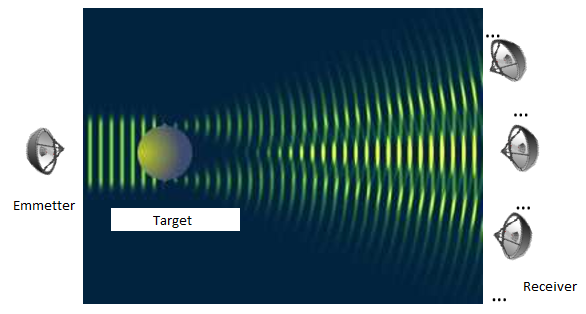
\includegraphics[scale=1,angle=0]{Images/Image1.PNG}
    \caption{General situation of our subject.}
    \label{fig:Image1}
\end{figure}

\bigskip

The first part will explain which equations have to be understood in order to get the analytic expression of the electromagnetic field coming from the object.
The second part will expose the different tools which have been created for the time frequency analysis that can be used for this project. In this part, some simple signals will be used in order to represent the results that can be obtained with these tools.
The last part will present the tools which have been developed in order to extract information from the time/frequency representation in order to find a correlation between the deformation of the object and the variation of the electromagnetic field.
